\renewcommand{\fieldheight}{48pt}
\begin{figure}[t]
  \centering
  \begin{tabular}{m{1pt}c@{\hspace{20pt}}m{1pt}c@{\hspace{20pt}}m{1pt}c}
    &\hspace{12pt}\small $t_{40}(\nu=3)$ && \hspace{12pt}\small\texttt{elliptical shell} && \hspace{12pt}\small\texttt{elliptical extreme} \\
    \raisebox{48pt}{\rotatebox{90}{\tiny magnitude $w_i$}} &
    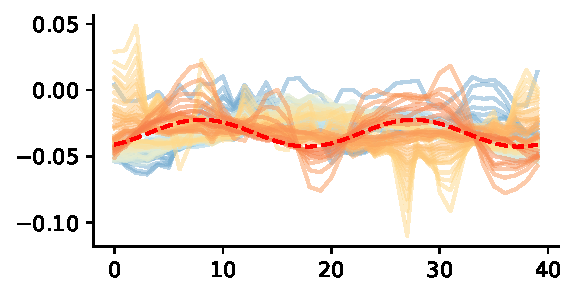
\includegraphics[height=\fieldheight]{rebuttal-figures/elliptical/t3.pdf} &
    \raisebox{48pt}{\rotatebox{90}{\tiny magnitude $w_i$}} &
    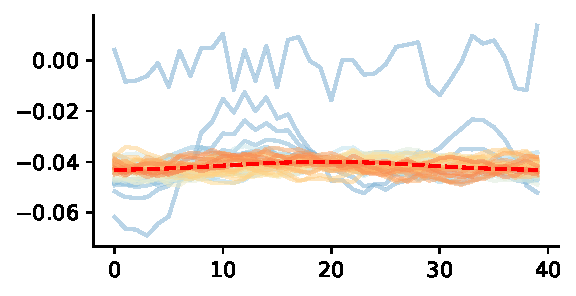
\includegraphics[height=\fieldheight]{rebuttal-figures/elliptical/shell.pdf} & 
    \raisebox{48pt}{\rotatebox{90}{\tiny magnitude $w_i$}} &
    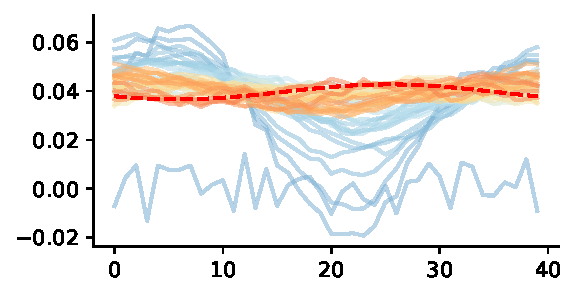
\includegraphics[height=\fieldheight]{rebuttal-figures/elliptical/extreme.pdf} \\
    \noalign{\vskip -40pt}
    &
    \hspace{12pt}\tiny dimension $i$ of weight $\mathbf{w}$ & &
    \hspace{12pt}\tiny dimension $i$ of weight $\mathbf{w}$ &&
    \hspace{12pt}\tiny dimension $i$ of weight $\mathbf{w}$ 
  \end{tabular}
  \caption{
    Evolution of receptive fields learned by the single-neuron model (\labelcref{item:single-neuron-model}), along with sinusoids fit to final states (red dashes) when trained on data from three elliptical distributions: $t_{40}(\nu=3)$ (\textbf{left}), the surface of an ellipse (\textbf{middle}), and a custom elliptical distribution that places its mass near the outside of an ellipse (\textbf{right}).
    In all cases, the learned receptive field is oscillatory (a sinusoid), as predicted by Proposition \ref{thm:elliptical}.
    The $\ell_2$ distances between the fitted oscillatory weights and empirical RFs, as a ratio of the $\ell_2$ norm of the empirical RFs, are (left) 9.77\%, (center) 3.75\%, and (right) 4.14\%.
    \emph{See \cref{sec:elliptical-experiments} for exposition.}
    }
    \label{fig:elliptical}
\end{figure}
